% Conceptual curves only: not measured, simulated, or fitted customer data.
\documentclass[tikz,border=4pt]{standalone}
\usepackage[T1]{fontenc}
\usepackage{lmodern}
\usetikzlibrary{arrows.meta}
\begin{document}
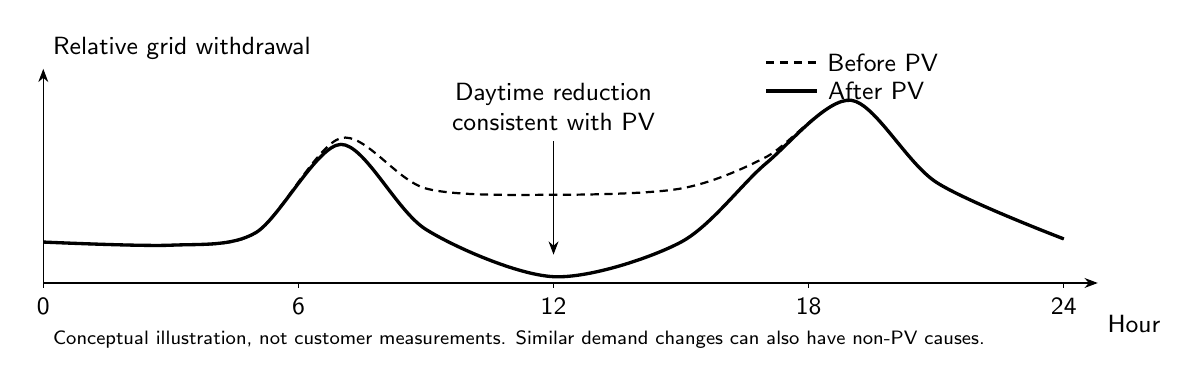
\begin{tikzpicture}[font=\sffamily\small,x=0.54cm,y=0.8cm]
\draw[-{Stealth}] (0,0) -- (24.8,0);
\draw[-{Stealth}] (0,0) -- (0,3.4) node[above right] {Relative grid withdrawal};
\node[anchor=west] at (24.8,-0.65) {Hour};
\foreach \x in {0,6,12,18,24} {\draw (\x,0) -- (\x,-0.08) node[below] {\x};}
\draw[densely dashed,thick] plot[smooth] coordinates {(0,0.65) (3,0.6) (5,0.8) (7,2.3) (9,1.5) (12,1.4) (15,1.5) (17,2.0) (19,2.9) (21,1.6) (24,0.7)};
\draw[very thick] plot[smooth] coordinates {(0,0.65) (3,0.6) (5,0.8) (7,2.2) (9,0.85) (12,0.1) (15,0.65) (17,1.9) (19,2.9) (21,1.6) (24,0.7)};
\node[align=center] at (12,2.8) {Daytime reduction\\consistent with PV};
\draw[-{Stealth}] (12,2.25) -- (12,0.45);
\draw[densely dashed,thick] (17,3.5) -- (18.2,3.5) node[right] {Before PV};
\draw[very thick] (17,3.05) -- (18.2,3.05) node[right] {After PV};
\node[font=\sffamily\scriptsize,anchor=west] at (0,-0.9) {Conceptual illustration, not customer measurements. Similar demand changes can also have non-PV causes.};
\end{tikzpicture}
\end{document}
